
%%%%%%%%%%%%%%%%%%%%%%%%%%%%%%%%%%%%%%%%%
% Dreuw & Deselaer's Poster
% LaTeX Template
% Version 1.0 (11/04/13)
%
% Created by:
% Philippe Dreuw and Thomas Deselaers
% http://www-i6.informatik.rwth-aachen.de/~dreuw/latexbeamerposter.php
%
% This template has been downloaded from:
% http://www.LaTeXTemplates.com
%
% License:
% CC BY-NC-SA 3.0 (http://creativecommons.org/licenses/by-nc-sa/3.0/)
%
%%%%%%%%%%%%%%%%%%%%%%%%%%%%%%%%%%%%%%%%%

%----------------------------------------------------------------------------------------
%	PACKAGES AND OTHER DOCUMENT CONFIGURATIONS
%----------------------------------------------------------------------------------------

\documentclass[final,hyperref={pdfpagelabels=false}]{beamer}

\usepackage[orientation=portrait,size=a1,scale=1.4]{beamerposter} % Use the beamerposter package for laying out the poster with a portrait orientation and an a0 paper size

\usetheme{GeoURV} % Use the GeoURV theme supplied with this template

\usepackage[english, catalan]{babel} % English language/hyphenation

\usepackage{apacite}
\usepackage{natbib}
\usepackage{amsmath,amsthm,amssymb,latexsym} % For including math equations, theorems, symbols, etc
\usepackage{lipsum}

%\usepackage{times}\usefonttheme{professionalfonts}  % Uncomment to use Times as the main font
%\usefonttheme[onlymath]{serif} % Uncomment to use a Serif font within math environments

\boldmath % Use bold for everything within the math environment

\usepackage{booktabs} % Top and bottom rules for tables

\graphicspath{{figures/}} % Location of the graphics files



\title{\LARGE Prediction on cosmological parameters using weak gravitational lensing}
\author{Constanza Espinoza, Vicente Pedreros, Daniela Grandón, Domenico Sapone}
\institute{Departamento de Fisica, Facultad de Ciencias Físicas y Matemáticas
, Universidad de Chile}

\newcommand{\leftfoot}{maria.espinoza.d@ug.uchile.cl}
\newcommand{\rightfoot}{vicente.pedreros@ug.uchile.cl}


\begin{document}

\begin{frame}[t] % The whole poster is enclosed in one beamer frame

\begin{columns}[t] % The whole poster consists of two major columns, each of which can be subdivided further with another \begin{columns} block - the [t] argument aligns each column's content to the top

\begin{column}{.02\textwidth}\end{column} % Empty spacer column

\begin{column}{.465\textwidth} % The first column

%------------
% OBJECTIVES
%------------
\begin{block}{Abstract}
% The estimation of the expected performance of experiments, by prediction of constraints in cosmological parameters, has so far relied on various individual methodologies and numerical implementations, which were developed for different observational probes. \\ 
The Euclid mission aims at understanding the accelerated expansion of the universe and what is the nature of the source responsible for this acceleration. Based on the work done on \textit{Euclid Preparation}, we aim to obtain estimates on the uncertainties of the cosmological parameters $\Omega_{m,0}$, $h$, $n_s$, $\sigma_8$, using fisher matrix forecasts, applied to weak lensing phenomenons.

\end{block}

%--------------
% INTRODUCCIÓ
%--------------
\begin{block}{Introduction}
	Assuming the spatially flat $\Lambda$\textbf{CDM} model as a baseline of this work, we can describe our model by a minimal set of parameters:
\begin{itemize}
    \item $\Omega_{m,0}$, the total matter energy densities at present time.
    \item $h$, the dimensionless Hubble parameter.
    \item $n_s$, the spectral index of the primordial density power spectrum.
    \item $\sigma_8$, the rms of present-day linearly evolved density fluctuations in spheres of $8h^{-1}$Mpc.
\end{itemize}
The Hubble parameter can be expressed as a function of redshift $H(z) = H_0 E(z)$, where is the Hubble parameter today and the proper distance function $E(z)$ can be expressed as:
$$ E(z) = \sqrt{\Omega_{m,0}(1+z)^3 +\Omega_{\Lambda,0}+ \Omega_{K,0}(1+z)^2}$$
where $\Omega_{\Lambda,0}=1-\Omega_{m,0}$, since for spatially flat cosmology the effective curvature density is zero. In addition we define the comoving distance to an object at redshift $z$ as:
$$r(z) = \frac{c}{H_0}\int_{0}^{z} \frac{dz}{E(z)}$$

which factors out the expansion of the universe today, providing a distance that does not change in time due to the expansion of space.

Finally, the matter power spectrum (mps) describes the density contrast of the universe as a function of the wave number and the redshift. It's depicted as: 
$$P_{\delta \delta}(k,z) = \left(\frac{\sigma _8}{\sigma _N}\right)^2\left[\frac{D(z)}{D(z=0)}\right]^2 T_m^2(k)k^{n_s}$$


%\begin{figure}
%
\includegraphics[width=0.5\linewidth]{placeholder.jpg}
%\caption{Peu de la figura}
%\end{figure}



\end{block}

\begin{block}{Weak Lensing}


We model the first of the five quantities that comes from the W.L observable; \textbf{The cosmic shear power spectrum}, i.e is the change in the ellipticity of the image of background galaxy, caused by the lensing effect of large-scale structure along the line of sight. The correlation function that describe this phenomenon is:
$$C_{ij}^{\gamma\gamma}(\ell)\simeq \frac{c}{H_0}\int dz\frac{W_i^\gamma(z)W_j^\gamma(z)}{E(z)r²(z)}P_{\delta\delta}\left[\frac{\ell + 1/2}{r(z)},z\right]$$ where $i$ and $j$ identify pairs of redshift bins, the mps is evaluated at $k=k_\ell(z)\equiv(\ell+1/2)/r(z)$ (Limber approximation), and the weight functions $W_i^\gamma(z)$ are defined as 


$$W_i^\gamma(z) = \frac{3}{2}\left(\frac{H_0}{c}\right)^2\Omega_{m,0}(1+z)r(z)
\int_z^{z_{max}}dz'n_i(z')\left[1-\frac{\tilde{r}(z)}{\tilde{r}(z')}\right]$$ 

where the integral is also known as the window function ($\tilde{W}_i(z)$). The term $n_i(z)$ corresponds to the number density distribution of the observed galaxies in the ith bin. %$$\tilde{W}_i(z)=\int_z^{z_{max}}dz'n_i(z')\left[1-\frac{\tilde{r}(z)}{\tilde{r}(z')}\right]$$

    
\end{block}
\begin{block}{Fisher Matrix}

Assuming the signal is the mean power spectrum, the Fisher matrix reads
$$F_{\alpha\beta}=\sum_{\ell=\ell_{min}}^{\ell{max}}\sum_{ij,mn}\frac{\partial C_{ij}^{\epsilon\epsilon}(\ell)}{\partial \theta_\alpha}\text{Cov}^{-1}[C_{ij}^{\epsilon\epsilon}(\ell), C_{mn}^{\epsilon\epsilon}(\ell)]
\frac{\partial C_{mn}^{\epsilon\epsilon}(\ell)}{\partial \theta_\beta}$$ 
and corresponds to the curvature of the logarithmic likelihood, describing how fast the likelihood falls around the maximum.
\end{block}
\end{column}


%-------------
% METODOLOGIA
%-------------
 % End of the first column

\begin{column}{.03\textwidth}\end{column} % Empty column

\begin{column}{.465\textwidth} % The second column
% %---------
% % RESULTS
% %---------
\vspace{10}\\

The covariance matrix is depicted as: $$Cov[C_{ij}^{\epsilon\epsilon}(\ell), C_{kl}^{\epsilon\epsilon}(\ell')]=\frac{C_{ik}^{\epsilon\epsilon} C_{jl}^{\epsilon\epsilon}(\ell') + C_{il}^{\epsilon\epsilon}(\ell)C_{lk}^{\epsilon\epsilon}(\ell')}{(2l+1)f_{sky}\Delta \ell}\delta_{ll'}^K$$ where $f_{sky}$ is the fraction of surveyed sky and $\Delta \ell $ is the multipole bandwith.


 Finally it's possible to calculate the expected marginalized $1-\sigma$ error on the parameter $\theta_\alpha$ (left) and the unmarginalised expected errors (right)
$$\sigma_\alpha = \sqrt{(F^{-1})_{\alpha\alpha}}\,, \hspace{1cm} \sigma_\alpha =  \sqrt{1/F_{\alpha\alpha}}$$ accomplishing our main goal: the estimation of the uncertainties of the cosmological parameters.
%$$\frac{\partial C_{ij}^{\gamma\gamma}(\ell)}{\partial \theta_\mu} = \int_{z_{min}}^{z_{max}}dz\frac{\partial K_{ij}^{\gamma\gamma}(z)}{\partial \theta_\mu} P_{\delta\delta}[k_\ell(z),z] +\int_{z_{min}}^{z_{max}}dzK_{ij}^{\gamma\gamma}(z)\frac{\partial P_{\delta\delta}[k_\ell(z),z]}{\partial \theta_\mu}$$ 
%
%where 
%$K_{ij}^{\gamma\gamma}(z) =  \left[\frac{3}{2}\Omega_{m,0}(1+z)\right]²\left(\frac{H_0}{c}\right)³\frac{\tilde{W}_i^\gamma(z)\tilde{W}_j^\gamma(z)}{E(z)}$

%------------
% RESULTADINHO
%------------
\begin{block}{Results}
In order to obtain the cosmic shear power spectrum the mps is needed, which was obtained with CAMB \cite{p3} in two ways: by calling the CAMB interpolator directly (left) and by calling camb to obtain points of the mps and interpolate manually (right).
\begin{figure}
    \centering
    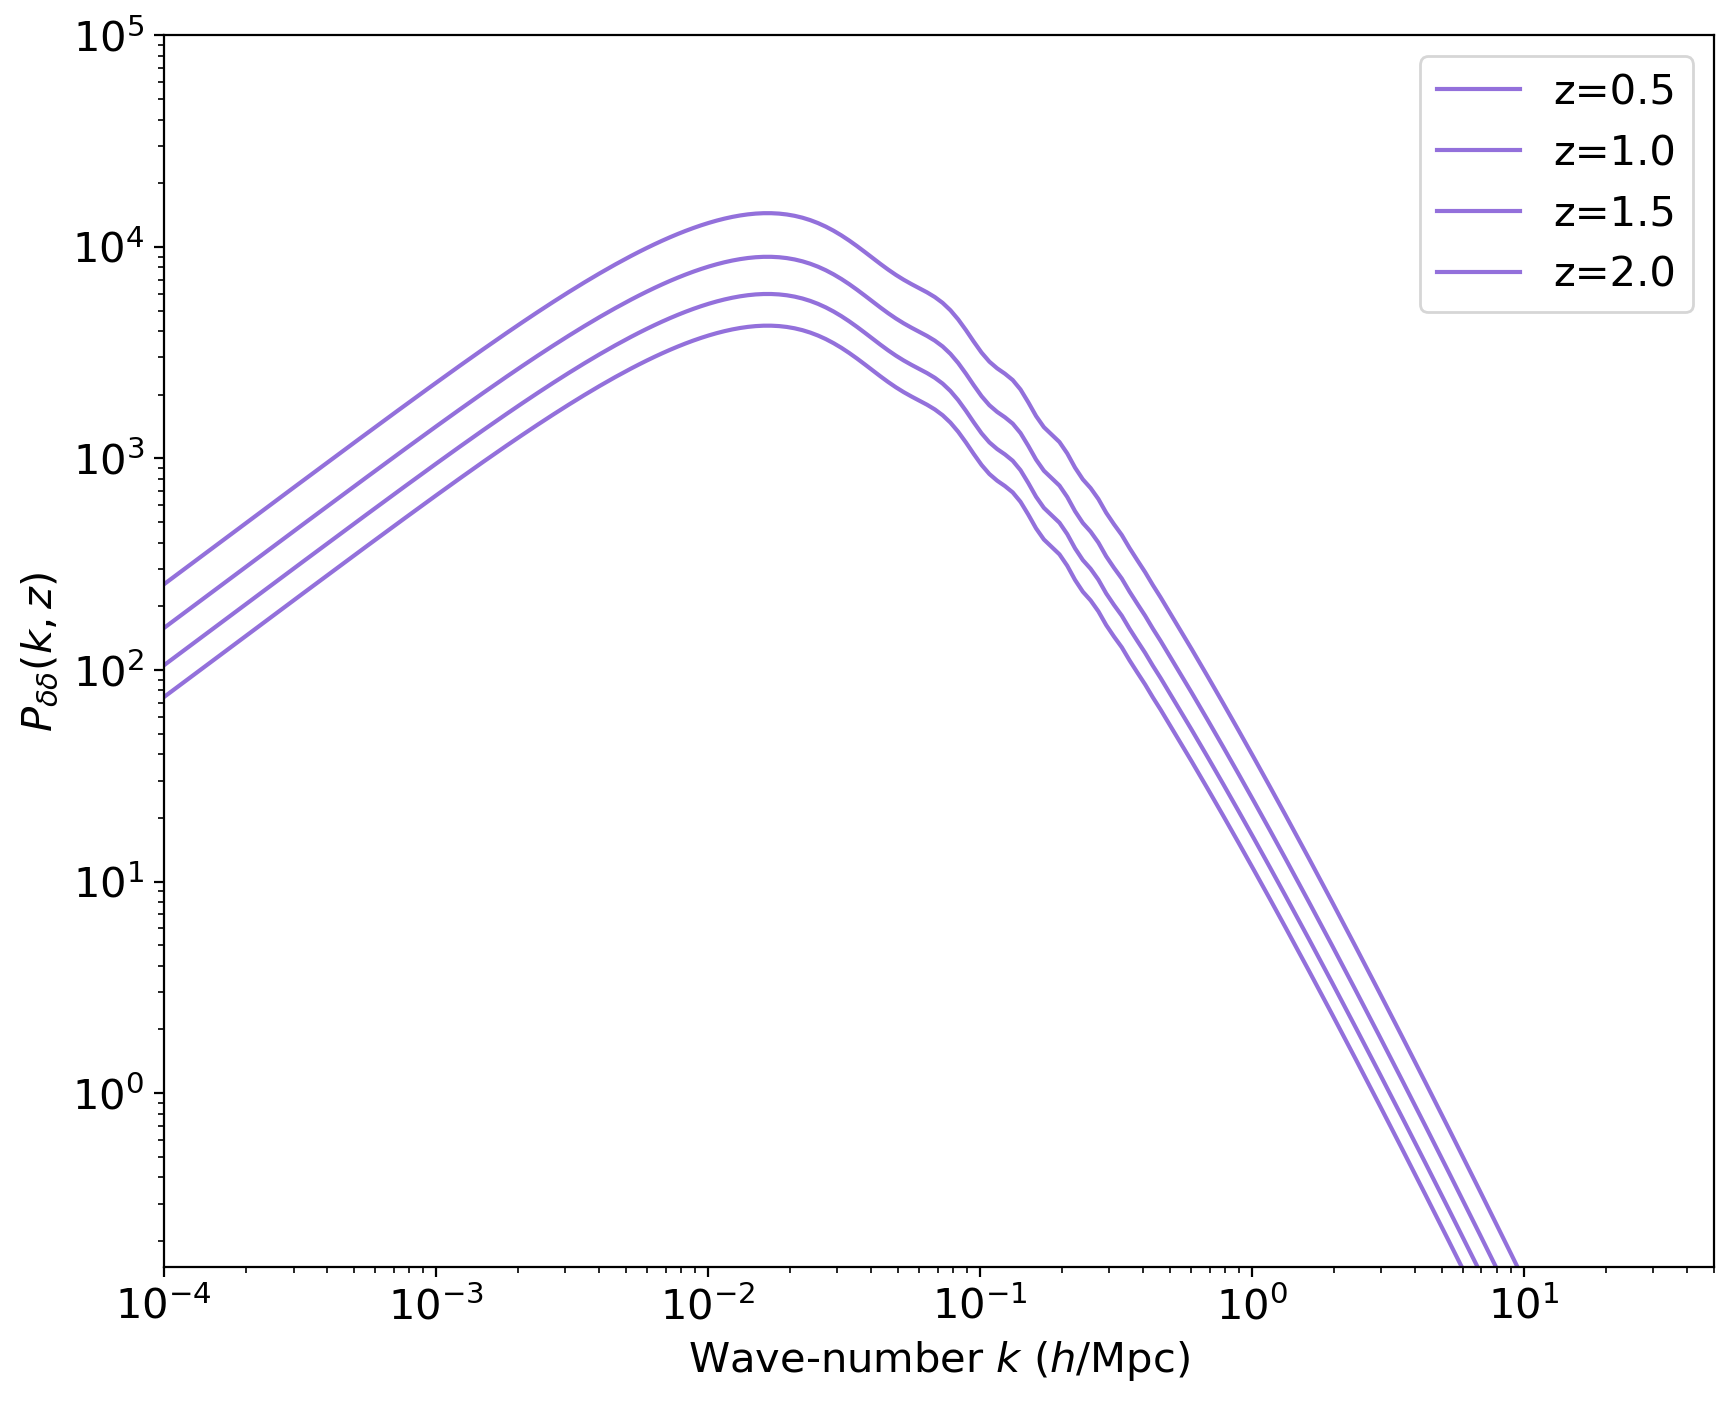
\includegraphics[width=0.45\textwidth]{fig_results/mps.png}
    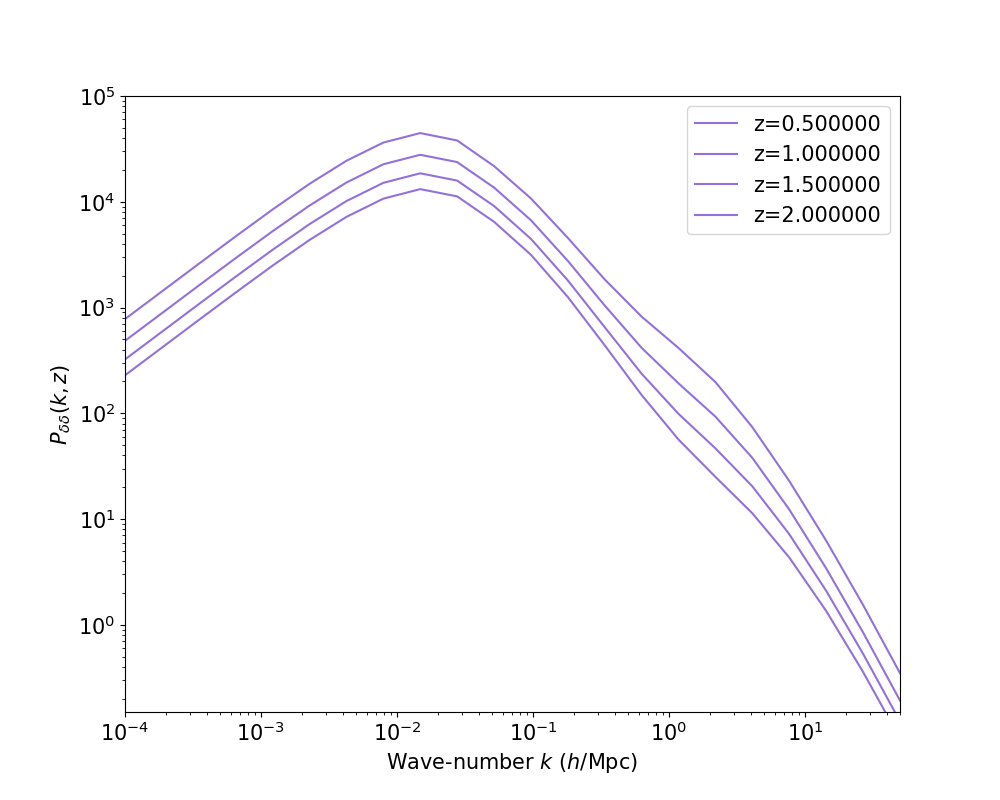
\includegraphics[width=0.5\textwidth]{fig_results/MPS.png}
    \label{mps}
\end{figure}

\begin{figure}
    \centering
    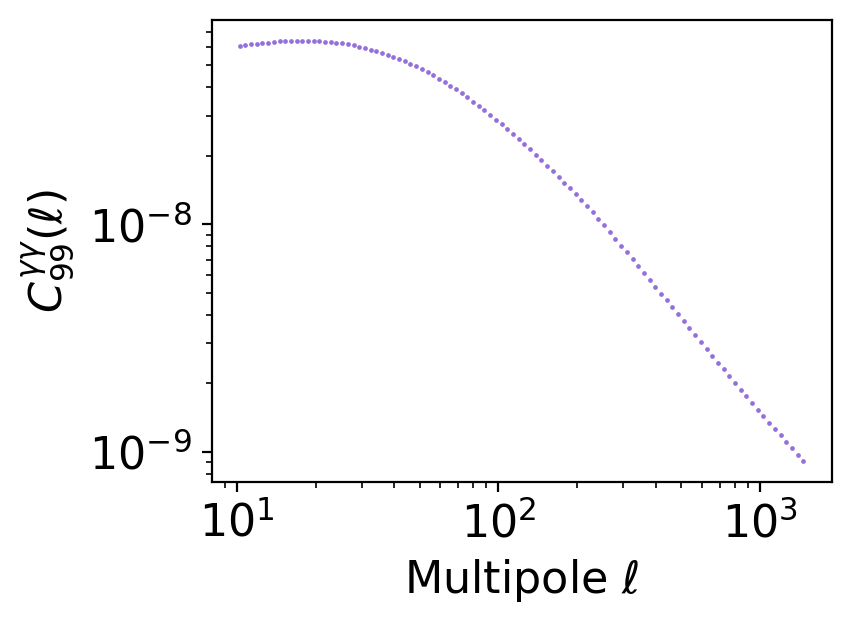
\includegraphics[width=0.47\textwidth]{fig_results/CSPS.png}
    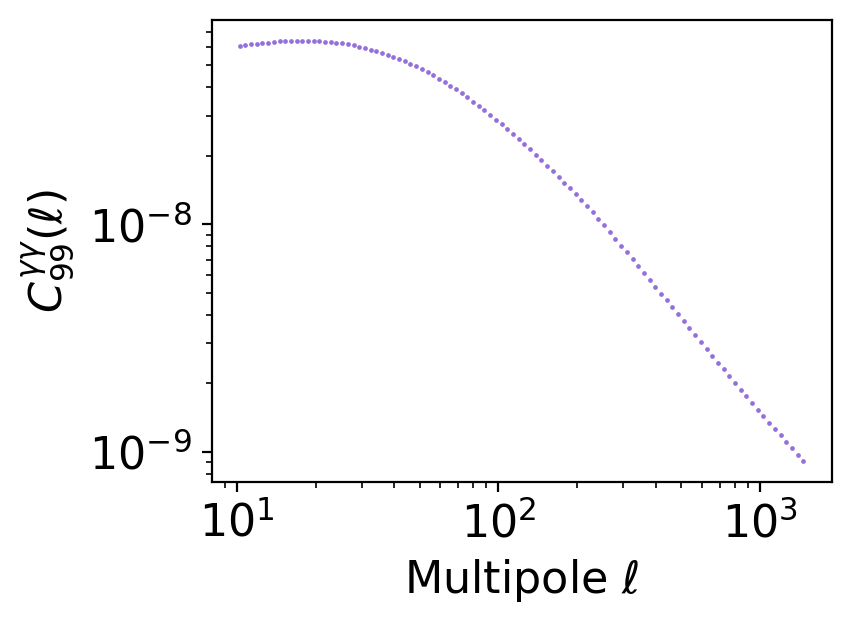
\includegraphics[width=0.47\textwidth]{fig_results/CSPS.png}
    \label{mps}
\end{figure}
The following is a comparison of the errors on the marginalised and unmarginalised cosmological parameters.

\begin{figure}
    \centering
    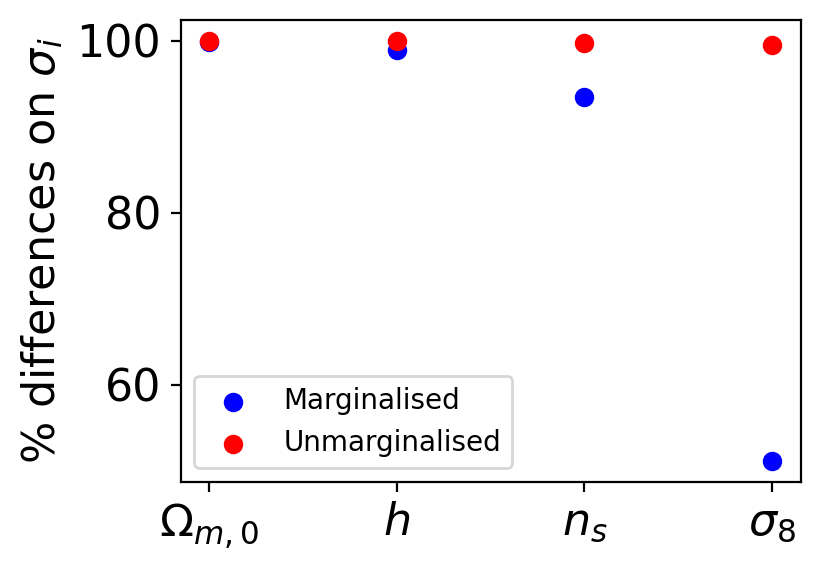
\includegraphics[width=0.45\textwidth]{fig_results/sigmas.png}
    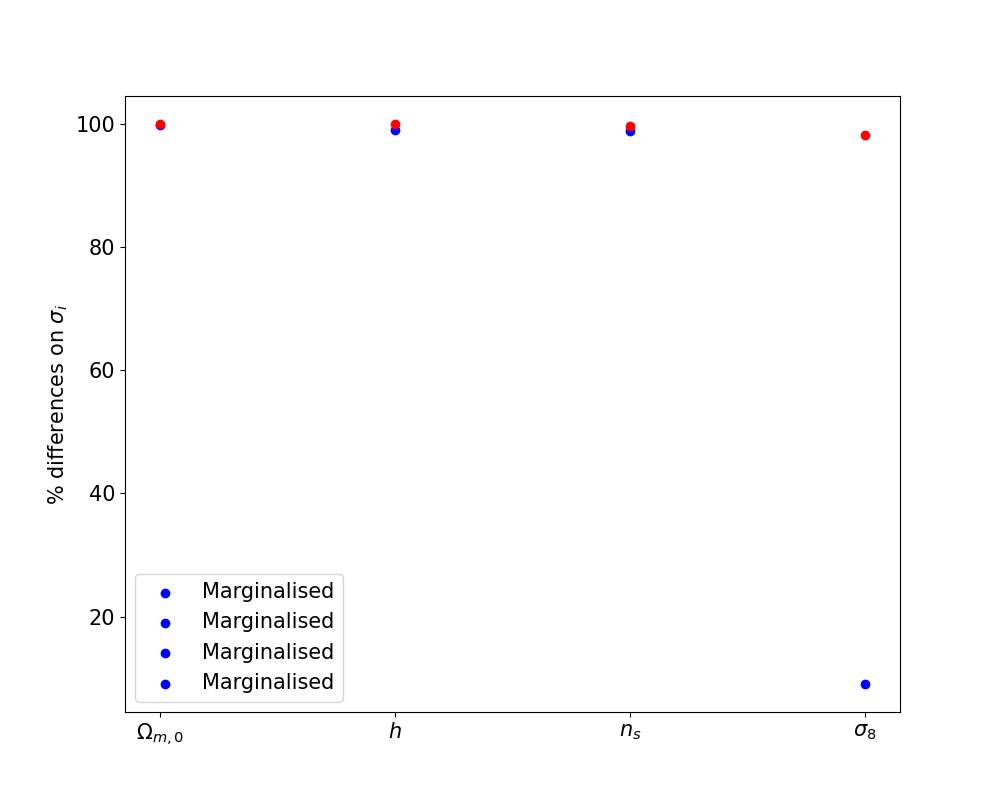
\includegraphics[width=0.5\textwidth]{fig_results/SIGMAS.png}
    \label{mps}
\end{figure}

\end{block}

%------------
% DISCUSSIÓ
%------------
\begin{block}{Discussion and Conclusions}
There are some minor differences in the mps fits. It is easy to notice that the mps obtained by manual interpolation decays more abruptly than the interpolation made by CAMB. However, the behaviour of the cosmic shear power spectrum is really similar for all the bins, since integration over redshift was performed.\\

When comparing to the errors obtained by the \textit{Euclid Collaboration}, we found that our errors were up to two orders of magnitude smaller. This could be explained by the fact that our covariance matrix had between 15 and 20 orders of magnitude more than expected. In the future, this will be studied carefully, along estimating other cosmological parameters (such as $\Omega_{b,o}$ $w_a$), consider the intrinsic alignment power spectrum, finding the appropiate shot noise and improving efficiency.

\end{block}
%-------------
% REFERÈNCIES
%-------------

\begin{block}{References}
        
%\nocite{*} % Insert publications even if they are not cited in the poster
\bibliographystyle{apacite}
\footnotesize{
\begin{thebibliography}{99}
            \bibitem[1]{p1} [1] Rachel Mandelbaum, (2017),
            \newblock Weak lensing for precision cosmology
            \newblock \emph{\url{arXiv:1710.03235v1}}
            
            \bibitem[2]{p2} [2] Euclid Collaboration, (2020),
            \newblock Euclid preparation: VII. Forecast validation for Euclid cosmological probes
            \newblock \emph{\url{arXiv:1910.09273v2}}

            \bibitem[3]{p3} [3] Lewis A, Challinor A,
            \newblock Code for Anisotropies in the Microwave Background (CAMB)
	    \newblock \emph{\url{https://camb.info}}
        \end{thebibliography}
    }

\end{block}

%----------------------------------------------------------------------------------------

\end{column} % End of the second column

\begin{column}{.015\textwidth}\end{column} % Empty spacer column

\end{columns} % End of all the columns in the poster

 % End of the enclosing frame
\end{frame}
\end{document}
